\documentclass[]{article}
\usepackage{polski}
\usepackage[utf8]{inputenc}
\usepackage{amsmath}
\usepackage{graphicx}
\usepackage{geometry}
\usepackage{float}

\geometry{a4paper, margin=0.6in}

%opening
\title{AMO - Projekt 2, zestaw danych saheart}
\author{Jakub Postępski}

\begin{document}

\maketitle



\section{Zadanie optymalizacji}
Metoda SVM pozwala na klasyfikację binarną danych. W metodzie  należy zminimalizować normę $|| \vec{w} ||$ opisujących hiperpłaszczyznę oddzielającą dane dla zbioru danych uczących. W projekcie przyjęto twardy margines pomiędzy danymi.

Zadanie prymalne można zapisać jako:

\[ \min || \vec{w} || \]
przy ograniczeniach:

\[ y_i(\vec{w}*\vec{x_i} - b)\]

Dla $i\in {1..n}$ gdzie $n$ to ilość próbek mamy: $\vec{x_i}$ to wsp. kolejnych próbek a $y_i \in {-1, 1}$ to wartości klasyfikatorów.

Zadanie dualne można zapisać jako:

\[ \min || f(c_i) ||  = -\sum_{i=1}^{n} + \frac{1}{2}\sum{i=1}{n}\sum_{j=1}^{n}y_ic_ix_ix_jy_jc_j\]

przy ograniczeniach:
\[\sum_{i=1}^{n}c_iy_i = 0\]
\[c_i >= 0 \]


W celu uzyskania klasyfikacji należy obliczyć:
\[\vec{w}\vec{x_i}-b\]

Do implementacji problemu odpowiednio prymalnego i dualnego wykorzystano funkcje \textit{fmincon} i \textit{quadprog} w programie Matlab. 

\section{Testowe dane losowe}
Wygenerowano (funkcja \textit{randn}) zbiór danych pięciowymiarowych o wielkości 20 próbek(rys. \ref{fig:blisko}). Przyporządkowano je do dwóch klas poprzez zamianę ostatniej współrzędnej (pierwsza klasa wartości dodatnie, druga ujemne). Rozwiązanie prymalne i dualnie wygenerowały ten sam wektor. Klasywikacja była całkowicie zgodna z przyporządkowaniem.

\begin{figure}[H]
	\centering
	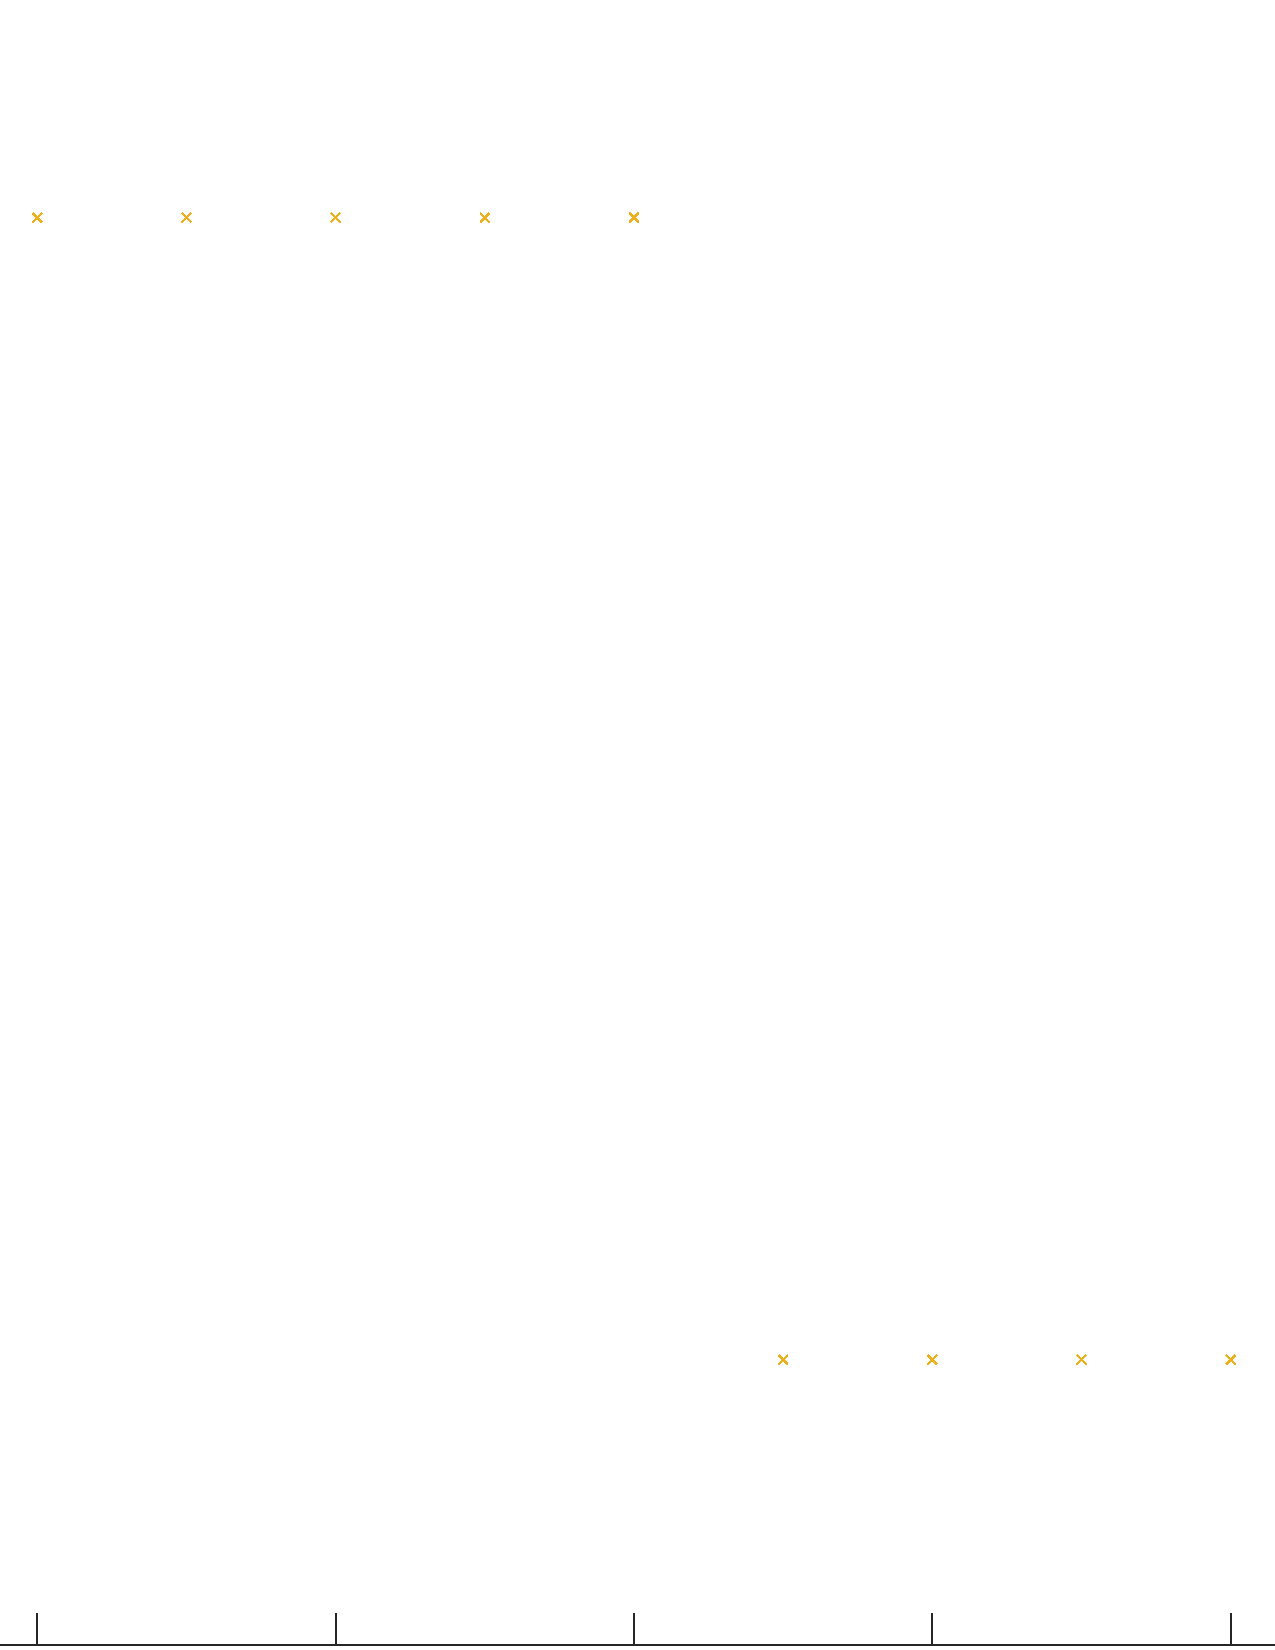
\includegraphics[width=0.9\linewidth]{dane_testowe}
	\caption{Wyniki klasyfikacji danych testowych}
	\label{fig:blisko}
\end{figure}


\section{Rzeczywiste dane}
Rzeczywiste dane (rys. \ref{fig:daleko})nie miały widocznej granicy pomiędzy płaszczyznami. Wykorzystanie optymalizacji problemu prymalnego pozwoliło na uzyskanie dokładności ok. 66 \%. Optymalizacja problemu dualnego nie udała się. 

\begin{figure}[H]
	\centering
	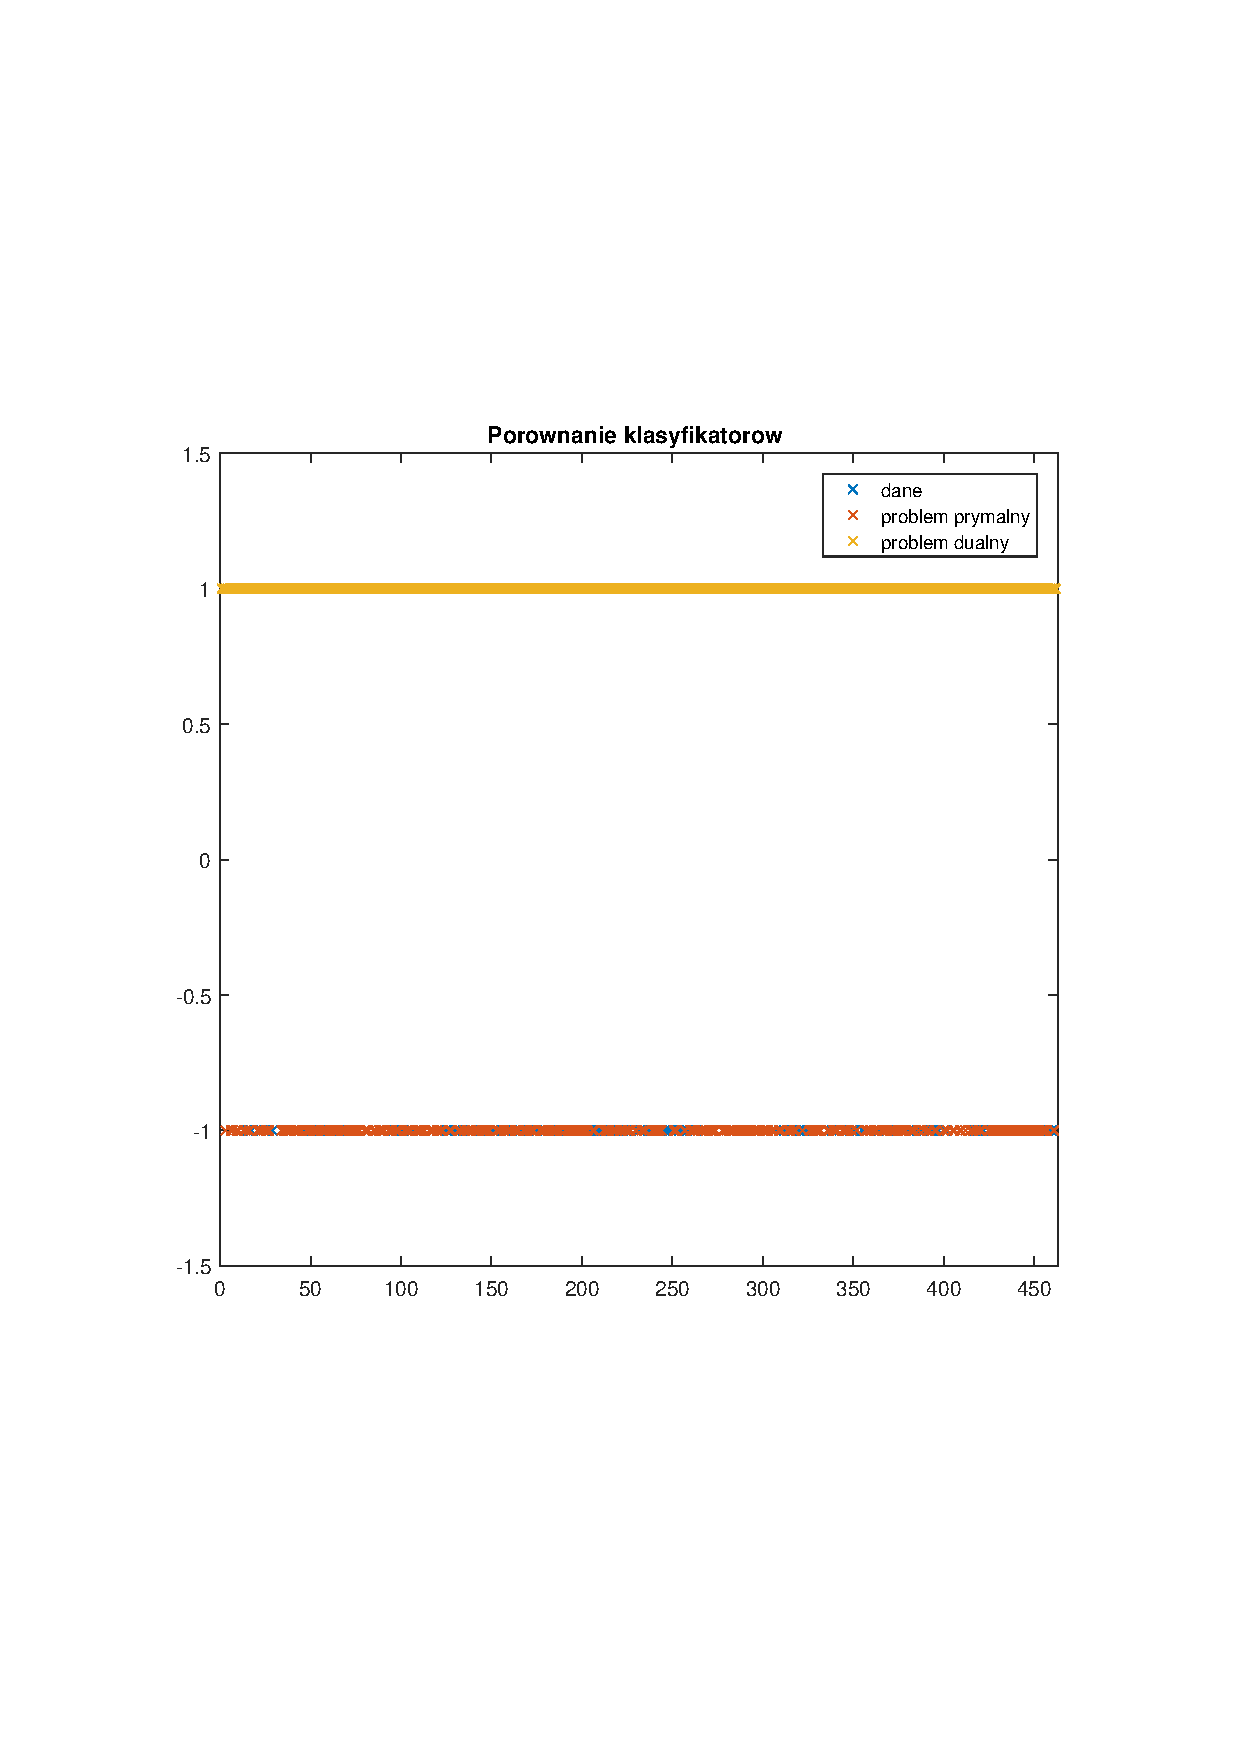
\includegraphics[width=0.9\linewidth]{dane_rzeczywiste}
	\caption{Wyniki klasyfikacji danych rzeczywistych}
	\label{fig:daleko}
\end{figure}

\section{Podsumowanie}
Zadanie prymalne pozwala na prostsze zapisanie problemu. Dodatkowo algortym jest bardziej skuteczny od zastosowanego w rozwiązaniu problemu dualnego. Problem prymalny można obliczać przy pomocy tych samych solwerów co problem dualny. W idealnym przypadku oba algorytmy dają to samo rozwiązanie.
\end{document}